\documentclass{beamer}
\usepackage[utf8]{inputenc}
\usepackage{media9}
\usepackage{lipsum}
\usepackage{amsmath}
\usepackage{amsfonts}
\usepackage{amssymb}
\usetheme{metropolis}
\usepackage{tcolorbox}
\usepackage{listings} 
\usepackage{lstlinebgcolor}
\usepackage{MnSymbol}
\usepackage{wasysym}
\usepackage{animate}

\lstset{% 
  basicstyle=\ttfamily\large,
  columns=fullflexible,
  escapeinside={(*@}{@*)},
  numbers=none,
  breaklines=true,
  numbersep=5pt,                   % how far the line-numbers are from the code
  numberstyle=\tiny\color{gray}, % the style that is used for the line-numbers
  numbersep=5pt,                   % how far the line-numbers are from the code
  % postbreak={\hbox{\raisebox{0ex}[0ex][0ex]\color{red}{\hookrightarrow}\space}}
  postbreak=\raisebox{0ex}[0ex][0ex]{\ensuremath{\rcurvearrowse\space}},
  keywordstyle=\color{blue},       % keyword style
  stringstyle=\color{red},     % string literal style
  language=Scala,
  % belowskip=0pt,
  % aboveskip=0pt,
  }

\definecolor{lightyellow}{RGB}{255,255,204}

\title{Spark}
\subtitle{Cluster computing}
\author{J. Fernando Sánchez, Joaquín Salvachúa, Gabriel Huecas }
\institute{Universidad Politécnica de Madrid}
\date{2016}



\newcommand{\btVFill}{\vskip0pt plus 1filll}


\begin{document}

\begin{frame}
\titlepage{}
\end{frame}
\begin{frame}[allowframebreaks]
\frametitle{Outline}
\tableofcontents
\end{frame}

\section{Background}

\begin{frame}
  \frametitle{LISP and functional programming}
  \begin{columns}
\column{0.5\textwidth}
  \begin{itemize}
  \item Higher level programming
  \item Avoid side effects
  \item Pattern matching
  \end{itemize}
\column{0.5\textwidth}
  
\includegraphics[width=\textwidth]{images/lisplogo.png}
\end{columns}
\end{frame}

\begin{frame}
  \frametitle{Scala}
  \begin{columns}
\column{0.5\textwidth}
  
\includegraphics[width=\textwidth]{images/scalalogo.png}
\column{0.5\textwidth}
  \begin{itemize}
    \item A \textit{better} Java
    \item Functional programming (optional)
    \item Actors for (coarse) concurrency
  \end{itemize}
\end{columns}
\end{frame}

\begin{frame}
  \frametitle{Docker}
  \begin{columns}
\column{0.5\textwidth}
  \begin{itemize}
    \item Easy and repeatable deployment
    \item Lots of pre-built images @ hub.docker.com
    \item Building block for other tools (swarm, compose, machine...)
  \end{itemize}
\column{0.5\textwidth}
  
\includegraphics[width=\textwidth]{images/docker_logo.png}
\end{columns}
\end{frame}

{
  \pagecolor{black}
  \usebackgroundtemplate{\vbox to \paperheight{\vfil\hbox to \paperwidth{\hfil
\includegraphics[height=\paperheight]{images/knowscala.jpg}\hfil}\vfil}}%

\begin{frame}[plain]
\end{frame}
}
{
  \pagecolor{black}
  \usebackgroundtemplate{\vbox to \paperheight{\vfil\hbox to \paperwidth{\hfil
\includegraphics[height=\paperheight]{images/knowbigdata.jpg}\hfil}\vfil}}%

\begin{frame}[plain]
\end{frame}
}
% \begin{frame}[plain]
%   \center
%   \huge{Show me}
% \end{frame}
{
  \pagecolor{white}
  \usebackgroundtemplate{\vbox to \paperheight{\vfil\hbox to \paperwidth{\hfil
\includegraphics[width=\paperwidth]{images/showme.png}\hfil}\vfil}}%
\begin{frame}[plain]

\end{frame}
}

\begin{frame}[fragile]
\frametitle{Word count in Wikipedia}

Problem: find the frequency each word is used in Wikipedia.

We have the text of all wikipedia in a text file\footnote{By happy coincidence, the first two lines are ``hi world'' and ``hi''}. It begins like this:

\begin{lstlisting}[backgroundcolor=\color{lightyellow},language={},postbreak={}, 
  breakautoindent=false, breakindent=0pt, breaklines]
hi world
hi
Scala (SKAH-lah)[9] is a general-purpose programming language. Scala has full support for functional programming and a strong static type system. Designed to be concise,[10] many of Scala's design decisions were inspired by criticism of Java's shortcomings.[8] 
\end{lstlisting}

\end{frame}

\begin{frame}[fragile]
\frametitle{Algorithm}

\begin{itemize}
  \item Read every line
  \item Chunk every line into words
  \item Count every occurrence
  \item For every word, sum its occurrences
\end{itemize}
\end{frame}

\begin{frame}[fragile]
\frametitle{Possible results of every step}
\begin{lstlisting}[language={},numbers=none,linebackgroundcolor={
      \btLstHL<1>{1}%
      \btLstHL<2>{2}%
      \btLstHL<3>{3,4}%
      \btLstHL<4>{5}%
    }]
(("hi world"), ("hi") ...)
List((hi, 1), (hi, 1), (world, 1) ...)
Map(hi ->(("hi", 1), (hi, 1)),
     world -> ((world, 1)) ...)
Map(hi-> 2, world -> 1 ...)
\end{lstlisting}
\end{frame}

\begin{frame}[fragile]
\frametitle{Running the scala shell}

We will use docker.

\begin{lstlisting}[language=bash,numbers=none]
docker run -it -v $PWD:Wikipedia.txt:Wiki \
            --rm williamyeh/scala
\end{lstlisting}
\end{frame}

\begin{frame}[fragile]
  \frametitle{Scala code}

%[linebackgroundcolor={
      % \btLstHL<1>{1} %
      % \btLstHL<2>{3} %
      % \btLstHL<3>{5} %
      % \btLstHL<4>{7} %
      % \btLstHL<5>{9} %
      % }]
\begin{lstlisting}[language=Scala,linebackgroundcolor={
      \btLstHL<1>{2}%
      \btLstHL<2>{3}%
      \btLstHL<3>{4}%
      \btLstHL<4>{5}%
      \btLstHL<5>{6,7}%
    }]
import scala.io.Source
val wiki = Source.fromFile("Wiki").getLines
wiki.flatMap(line=> line.split(" "))
      map(x=>(x, 1)).toList
      groupBy(x => x._1)
      map({case (k, v) =>
            (k, v.foldLeft(0)((a, b) => a+b._2)))
  \end{lstlisting}

\end{frame}

\begin{frame}

  \center
  {\huge Let's run it in the shell.}

\end{frame}

{
  \pagecolor{black}
  \usebackgroundtemplate{\vbox to \paperheight{\vfil\hbox to \paperwidth{\hfil
\includegraphics[height=\paperheight]{images/justwaithere.jpg}\hfil}\vfil}}%

\begin{frame}[plain]
\end{frame}
}

\begin{frame}
  \frametitle{Wikipedia is big}
  
\includegraphics[width=\textwidth]{images/outofmemory.jpg}
\end{frame}

\begin{frame}

  \center
  {\huge What happened?}

\end{frame}

\begin{frame}
  \frametitle{Limited resources}
  \begin{itemize}
  \item CPU limits our speed
    \begin{itemize}
    \item Multi-cores help...
    \item ...but real parallelism is \textbf{hard}
    \end{itemize}
  \item RAM limits how much data you can process at the same time
    \begin{itemize}
    \item What if you need more than 128GB?
    \item You could use more than one computer...
    \item ... but cluster computing is even harder than ``local'' parallelism
    \end{itemize}
  \item Functional programming helps a bit
  \end{itemize}
\end{frame}
\begin{frame}[plain]
  \center
  \huge But... this was supposed to be fun, wasn't it?
\end{frame}

\section{Introduction to Spark}

\subsection{What is Spark?}
{
  \pagecolor{white}
  \usebackgroundtemplate{\vbox to \paperheight{\vfil\hbox to \paperwidth{\hfil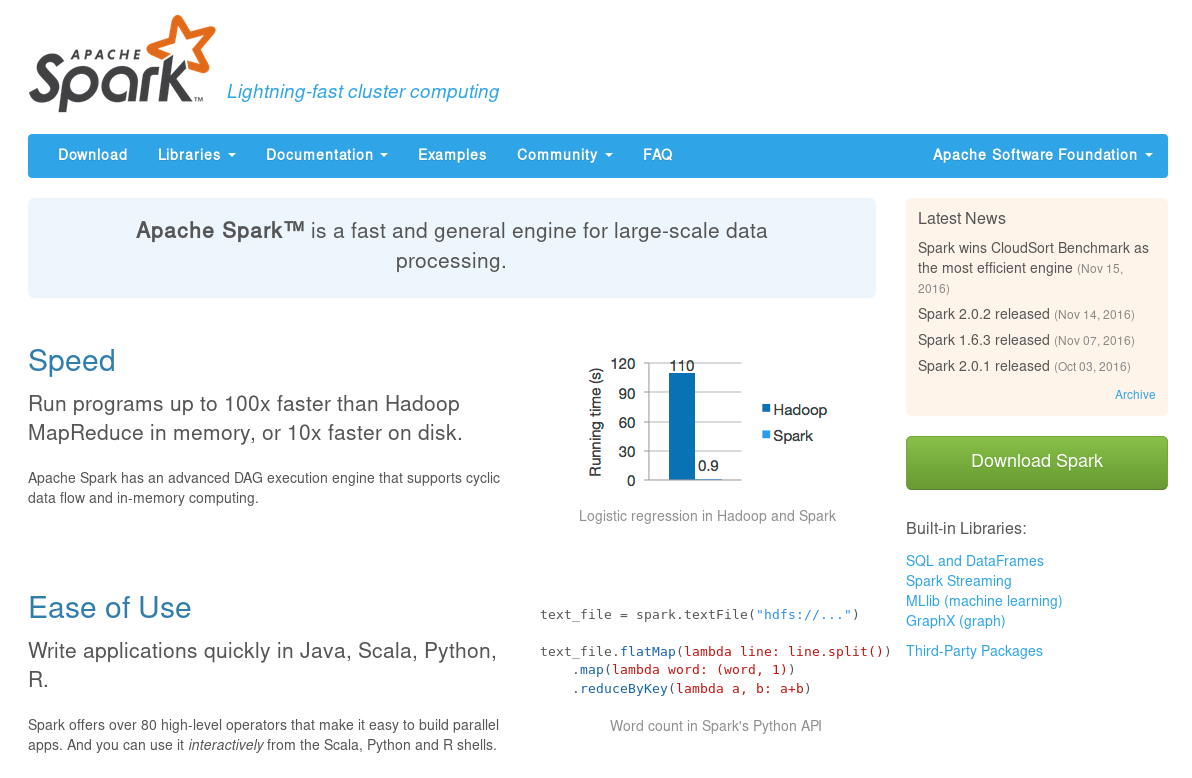
\includegraphics[width=\paperwidth]{images/sparkweb.png}\hfil}\vfil}}%
\begin{frame}[plain]

\end{frame}
}
\begin{frame}
\frametitle{Quick definition}
{\center {\huge Apache Spark™ is a fast and general engine for large-scale data processing.\footnote{\url{http://spark.apache.org}}}}

On top of that:
 \begin{itemize}
   \item Open source (Top-level Apache project)
   \item Plays well with other tools
   \end{itemize}
\end{frame}

\begin{frame}
  \frametitle{Architecture}
  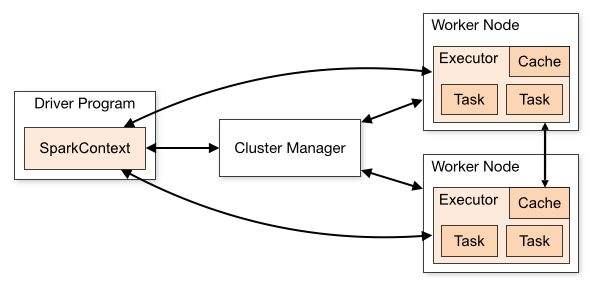
\includegraphics[width=\textwidth]{images/cluster-overview.png}
\end{frame}

\begin{frame}
  \frametitle{Programs}
  \center
  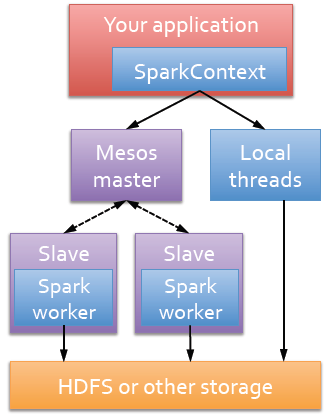
\includegraphics[height=.8\textheight]{images/sparkapp.png}
\end{frame}

\begin{frame}
  \frametitle{Ecosystem}
  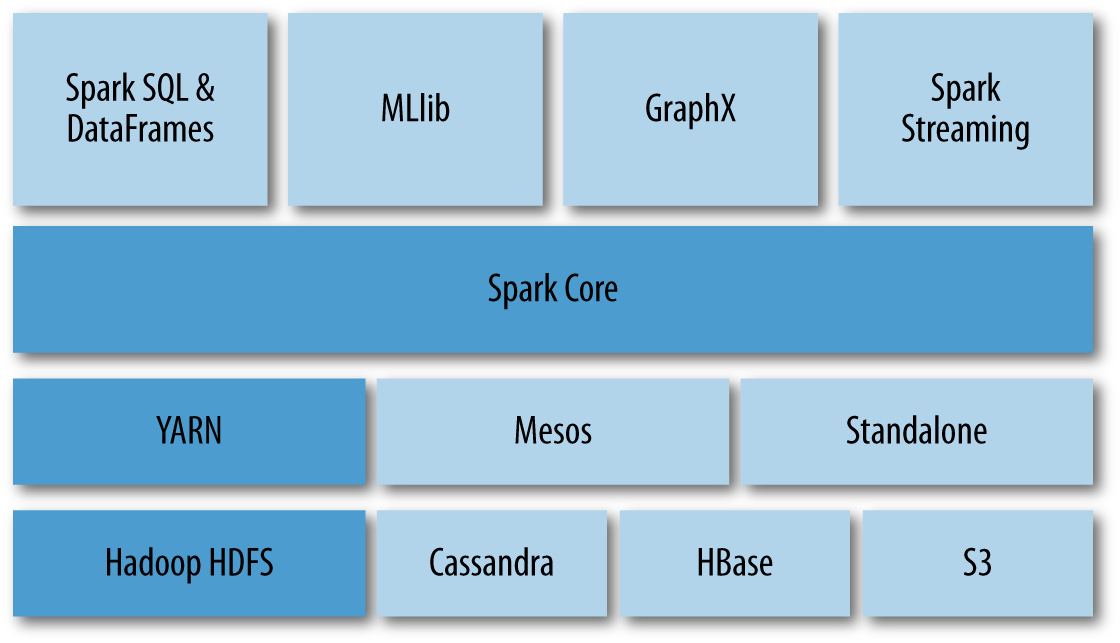
\includegraphics[width=\textwidth]{images/sparkecosystem.png}
\end{frame}

\subsection{vs MapReduce}

{
  \pagecolor{white}
  \usebackgroundtemplate{\vbox to \paperheight{\vfil\hbox to \paperwidth{\hfil
\includegraphics[width=\paperwidth]{images/hadoop-spark.png}\hfil}\vfil}}%

\begin{frame}[plain]
% \center
% \begin{tikzpicture}[remember picture,overlay]
% \node[at=(current page.center)] {
%   
\includegraphics[height=\paperheight]{images/justwaithere.jpg}
% };
% \end{tikzpicture}  
\end{frame}
}

\begin{frame}
\frametitle{Comparison to MapReduce}
\begin{itemize}
  \item In-memory data
    \begin{itemize}
      \item Less i/o overhead
      \item Faster operations
      \item Caching
    \end{itemize}
  \item Better for recursive tasks (e.g. machine learning)
  \item Some libraries are dropping MapReduce support
\end{itemize}
\end{frame}

  \begin{frame}
    \frametitle{Contributors to Spark/Hadoop 2014}
    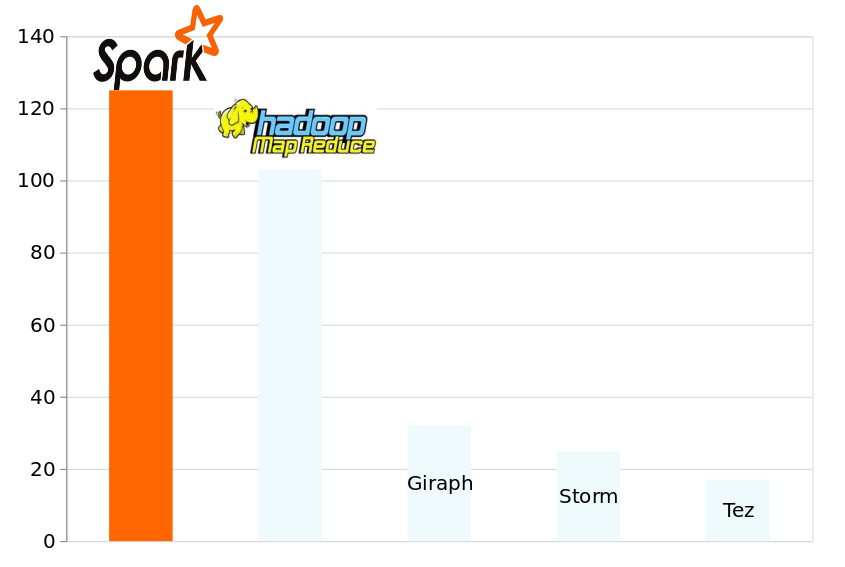
\includegraphics[width=\textwidth]{images/hadoopsparkcontribs.png}
  \end{frame}

\begin{frame}
\frametitle{Project status}
\center 

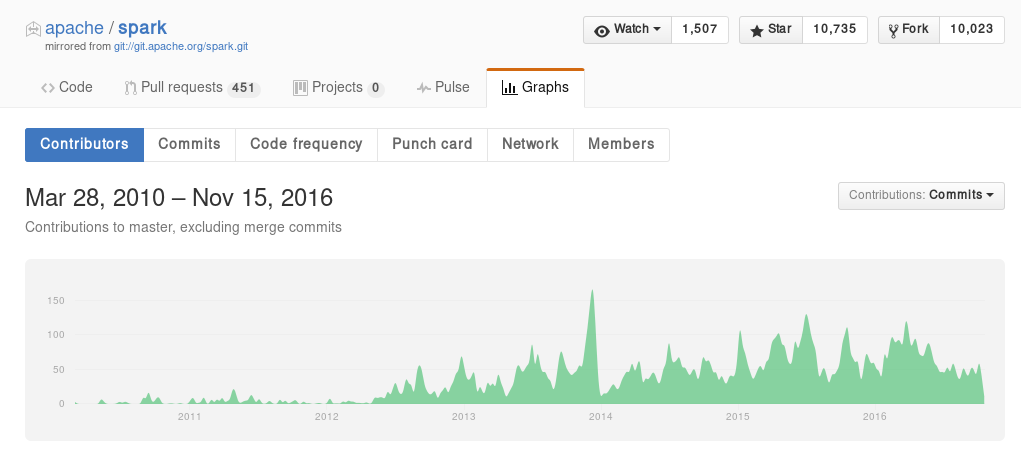
\includegraphics[width=\textwidth]{images/sparkgh.png}


\includegraphics[height=.35\textheight]{images/contributors.png}
\end{frame}

\subsection{Key concepts}

\begin{frame}
\frametitle{Overview}
  % {\huge Two core concepts}
  % \vfill
\begin{columns}[t]
    \column{0.5\textwidth}
    Data (RDDs/Datasets)
    
    \begin{itemize}
    \item RDD: Resilient Distributed Dataset
    \item Collections of objects spread across a cluster, stored in RAM or on Disk
    \item Built through parallel transformations
    \item Automatically rebuilt on failure
    \end{itemize}
    \column{0.5\textwidth}
    Operations
    \begin{itemize}
    \item Transformations (e.g. group, map, groupBy)
    \item Actions (e.g. count, collect, save)
    \end{itemize}
\end{columns}
\end{frame}

\begin{frame}
\frametitle{Transformations and actions}
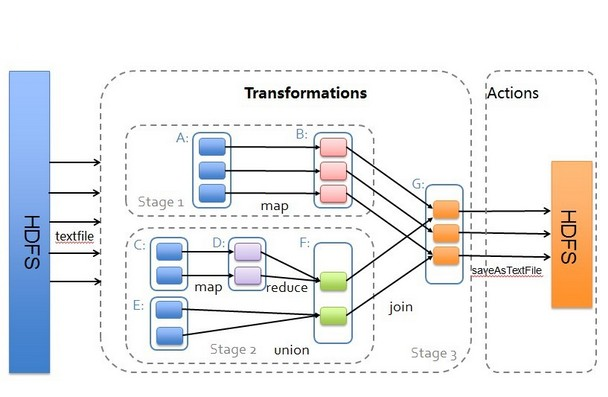
\includegraphics[width=\textwidth]{images/sparktransformations.png}
\end{frame}


\begin{frame}
  \frametitle{RDDs vs Datasets}
    Datasets are the future
    \begin{itemize}
      \item More memory efficient
      \item Libraries dropping support for RDDs
    \end{itemize}

\end{frame}
\begin{frame}
  \frametitle{RDDs vs Datasets}

    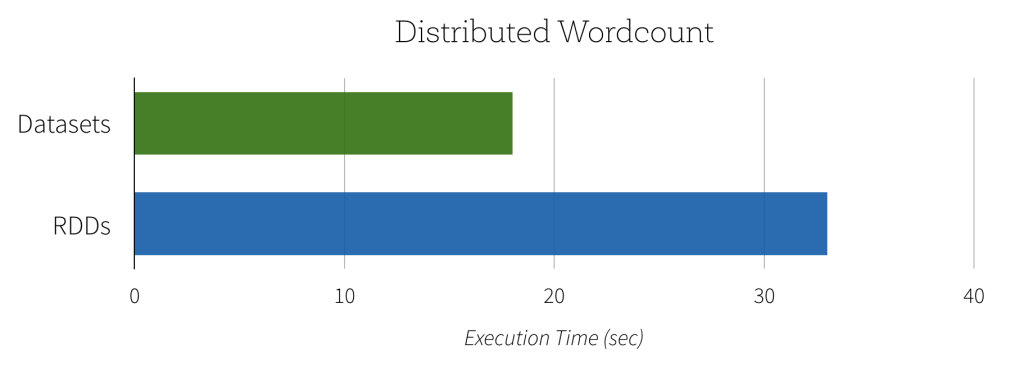
\includegraphics[width=\textwidth]{images/performance-wordcount-databricks.png}

    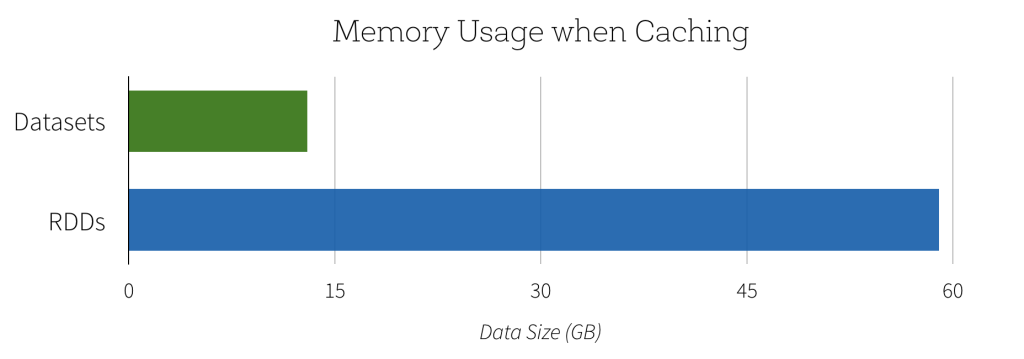
\includegraphics[width=\textwidth]{images/Memory-Usage-when-Caching-Chart-databricks.png}
  \end{frame}

\begin{frame}[fragile]
  \frametitle{Language support}
\vspace{-2em}
    \begin{lstlisting}[title=Scala]
val lines = sc.textFile(...)
lines.filter(x => x.contains("ERROR")).count()
\end{lstlisting}
    \begin{lstlisting}[title=Python,language=Python]
lines = sc.textFile(...)
lines.filter(lambda s: "ERROR" in s).count()
\end{lstlisting}
    \begin{lstlisting}[title=Java,language=Java]
      Removed, to keep the slides clean :)
\end{lstlisting}

\center
sc is the Spark Context (more or this later)
\end{frame}

\begin{frame}
  \frametitle{Different flavors}
  \begin{center}
    \begin{tabular}{ | l | c | c | c |}
      \hline
      Language & App & REPL & Performance \\ \hline
      Scala & Yes & Yes & \huge{\color{green}\smiley} \\
      Java & Yes & No & \huge{\color{green}\smiley} \\
      Python & Yes & Yes & \huge{\color{yellow}\smiley}\\ \hline
    \end{tabular}
  \end{center}
The Read-eval-print-loop (REPL) is the easiest way to get started and explore datasets. It is just a special Spark application that accepts user input (scala code).
  
\end{frame}

\section{Working with RDDs}

\begin{frame}[fragile]
\frametitle{Creation}

\begin{lstlisting}[title=From normal data structures,numbers=none]
val nums = sc.parallelize(List(1, 2, 3))
val cont = sc.parallelize(List(("a", 1),
                                   ("a", 1),
                                   ("b", 3)))
\end{lstlisting}

\begin{lstlisting}[title=From distributed/local sources,numbers=none]
sc.textFile('myfile')
\end{lstlisting}

\vfill
\vfill
Note: sc is the spark context in the Spark interpreter

\end{frame}

%  #################################
%  Starts Collect
%  #################################

\begin{frame}[fragile]
\frametitle{Operations: collect}
\only<1>{
  \btVFill
{\huge\ttfamily collect()}
}

\begin{onlyenv}<2->

\btVFill

\begin{lstlisting}[numbers=none,basicstyle=\Large\ttfamily,title={Runs any pending transformation and returns the real values},linebackgroundcolor={\btLstHL{1,3}}]
nums.collect()
> List(1, 2, 3) 
cont.collect()
> List((a, 1), (a, 1), (b, 3))
\end{lstlisting}

\end{onlyenv}

\btVFill

Reminder:
\begin{lstlisting}[numbers=none,linebackgroundcolor={\color{lightyellow}}]
nums: List(1, 2, 3)
cont: List(("a", 1), ("a", 1), ("b", 3))
\end{lstlisting}

\end{frame}

%  #################################
%  Ends Collect
%  #################################

%  #################################
%  Starts Take
%  #################################

\begin{frame}[fragile]
\frametitle{Operations: take}
\only<1>{
  \btVFill
{\huge\ttfamily take(N)}
}

\begin{onlyenv}<2>

\btVFill

\begin{lstlisting}[title=Returns the N first elements,basicstyle=\Large\ttfamily,linebackgroundcolor={\btLstHL<2>{1,3}}]
nums.take(2) 
>  List(1, 2)
cont.take(1) 
>  List((a, 1))
\end{lstlisting}

\end{onlyenv}

\btVFill

Reminder:
\begin{lstlisting}[numbers=none,linebackgroundcolor={\color{lightyellow}}]
nums: List(1, 2, 3)
cont: List(("a", 1), ("a", 1), ("b", 3))
\end{lstlisting}

\end{frame}

%  #################################
%  Ends Take
%  #################################

%  #################################
%  Starts Count
%  #################################

\begin{frame}[fragile]
\frametitle{Operations: count}
\only<1>{
  \btVFill
{\huge\ttfamily count()}
}

\begin{onlyenv}<2>

\btVFill

\begin{lstlisting}[title=Returns the number of elements in a collection,basicstyle=\Large\ttfamily,linebackgroundcolor={\btLstHL<2>{1,3}}]
nums.count() 
>  3
cont.count() 
>  3
\end{lstlisting}

\end{onlyenv}

\btVFill

Reminder:
\begin{lstlisting}[numbers=none,linebackgroundcolor={\color{lightyellow}}]
nums: List(1, 2, 3)
cont: List(("a", 1), ("a", 1), ("b", 3))
\end{lstlisting}

\end{frame}

%  #################################
%  Ends Count
%  #################################
%  #################################
%  Starts filter
%  #################################

\begin{frame}[fragile]
\frametitle{Operations: filter}
  \btVFill
\only<1,2>{
{\huge\ttfamily filter(fn)}
  \btVFill
}

\begin{onlyenv}<2>
This time, we need to define a function.

Filter applies that function to every element, and returns those where the function returns true.

For example:

\end{onlyenv}
\begin{onlyenv}<2,3>
\begin{lstlisting}[basicstyle=\ttfamily\Large]
val fn = (x:Int)) => x > 1
\end{lstlisting}
\end{onlyenv}
\begin{onlyenv}<3>

\btVFill

\begin{lstlisting}[title=Return a list containing the values where the function returns true,linebackgroundcolor={\btLstHL<3>{1}},basicstyle=\ttfamily\Large]
nums.filter(fn) 
>  List(2, 3)
\end{lstlisting}
\end{onlyenv}

\btVFill

Reminder:
\begin{lstlisting}[numbers=none,linebackgroundcolor={\color{lightyellow}}]
nums: List(1, 2, 3)
cont: List(("a", 1), ("a", 1), ("b", 3))
\end{lstlisting}

\end{frame}

%  #################################
%  Ends filter
%  #################################

\begin{frame}[fragile]
  \frametitle{Quick aside: anonymous functions and underscores}

% Defining a function when it is only going to be used once is tedious and makes reading code harder.

\only<1,2>{
{\Large In scala, we can define ``anonymous functions'', also known as lambda functions.}
}

\pause

\vspace{-2em} % Avoid overlapping with footer
\begin{lstlisting}[basicstyle=\ttfamily\Large]
val fn = (x:Int)) => x > 1
cont.filter(fn)
\end{lstlisting}

\only<2>{
{\Large is equivalent to:}
}

\begin{lstlisting}[basicstyle=\ttfamily\Large]
cont.filter((x:Int) => x>1)
\end{lstlisting}

\pause

\only<3>{
{\Large Additionally, the scala compiler is smart enough to infer types in this example. Hence, we could simply write:}
}

\begin{lstlisting}[basicstyle=\ttfamily\Large]
cont.filter(x => x>1)
\end{lstlisting}

\pause

{\Large Furthermore, we could use underscores to replace arguments:}

\vspace{-2em}

\begin{lstlisting}[basicstyle=\ttfamily\huge]
cont.filter(_>1)
\end{lstlisting}

\end{frame}

\begin{frame}[fragile]
  \frametitle{Quick aside: anonymous functions and underscores}
  
{\large Every new argument in the lambda function represents a parameter
  
Hence, these two expresions are equivalent
}
  
\begin{lstlisting}[basicstyle=\ttfamily\huge]
_ + _
(x,y) => x+y
\end{lstlisting}


\end{frame}

\begin{frame}[fragile]
  \frametitle{Operations: filter}
  
\Large Our last example could be written more concisely as:

\vfill

\begin{lstlisting}[linebackgroundcolor={\btLstHL<1>{1}},basicstyle=\ttfamily\Large]
nums.filter(_>1) 
>  List(2, 3)
\end{lstlisting}

\end{frame}

\begin{frame}[fragile]
  \frametitle{Operations: filter}
  
\Large What would this filter do?

\vfill

\begin{lstlisting}[basicstyle=\ttfamily\Large,linebackgroundcolor={\btLstHL<1>{1}}]
cont.filter(_._1 == "a" && _._1 == 1) 
>  ???
\end{lstlisting}

\end{frame}

\begin{frame}[fragile]
  \frametitle{Operations: filter}
  

\begin{lstlisting}[basicstyle=\ttfamily\normalsize,language={}]
<console>:9: error: missing parameter type
for expanded function ((x$1, x$2) =>
x$1._1.$eq$eq(a).$amp$amp(x$2._1.$eq$eq(1)))
Note: The expected type requires a
one-argument function accepting a 2-Tuple.
\end{lstlisting}
\end{frame}

{
  \pagecolor{black}
  \usebackgroundtemplate{\vbox to \paperheight{\vfil\hbox to \paperwidth{\hfil
\includegraphics[height=\paperheight]{images/whatsparrow.jpg}\hfil}\vfil}}%

\begin{frame}[plain]
\end{frame}
}

\begin{frame}[fragile]
  \frametitle{Operations: filter}
  
Remember, each new underscore represents a new argument. So that expression expands to:

\begin{lstlisting}[language=TeX,basicstyle=\ttfamily\Large]
cont.filter((x, y) => x._1 == "a" &&
                   y._2 == 1) 
\end{lstlisting}
\end{frame}

\begin{frame}[fragile]
  \frametitle{Operations: filter}

The right expression is:

\begin{lstlisting}[basicstyle=\ttfamily\Large,linebackgroundcolor={\btLstHL<1>{1,2}}]
cont.filter(x => x._1 == "a" &&
                   x._2 == 1) 
> List((a, 1), (a, 1))
\end{lstlisting}
\end{frame}


%  #################################
%  Starts map
%  #################################

\begin{frame}[fragile]
\frametitle{Operations: map}
  \btVFill
\only<1>{
{\huge\ttfamily map(fn)}
  \btVFill
}

\begin{onlyenv}<2>
\begin{lstlisting}[title=Apply a function to every item in the list,basicstyle=\Large\ttfamily,linebackgroundcolor={\btLstHL<2>{1,3}},basicstyle=\ttfamily\Large]
cont.map(x._2) 
>  List(1, 1, 3)
nums.map(_*3) 
>  List(3, 6, 9)
\end{lstlisting}
\end{onlyenv}

Reminder:
\begin{lstlisting}[numbers=none,linebackgroundcolor={\color{lightyellow}}]
nums: List(1, 2, 3)
cont: List(("a", 1), ("a", 1), ("b", 3))
\end{lstlisting}

\end{frame}


%  #################################
%  Ends map
%  #################################
%  #################################
%  Starts reduce
%  #################################

\begin{frame}[fragile]
\frametitle{Operations: reduce}
  \btVFill
\only<1>{
{\huge\ttfamily reduce(fn)}
  \btVFill
}

\begin{onlyenv}<2>

\btVFill

\begin{lstlisting}[title={Merge elements with an associative function (concisely)},basicstyle=\Large\ttfamily,linebackgroundcolor={\btLstHL<2>{1,3,4}}]
nums.reduce(_+_) 
>  6
cont.reduce((x, y) => (x._1+y._1,
                          x._2*y._2) 
>  (aab, 3)
\end{lstlisting}
\end{onlyenv}

\btVFill

Reminder:
\begin{lstlisting}[numbers=none,linebackgroundcolor={\color{lightyellow}}]
nums: List(1, 2, 3)
cont: List(("a", 1), ("a", 1), ("b", 3))
\end{lstlisting}

\end{frame}

%  #################################
%  Ends reduce
%  #################################

\begin{frame}[fragile]
\frametitle{Operations}
\begin{onlyenv}<1>
  \btVFill
{\huge\ttfamily groupByKey()}
  \btVFill
\end{onlyenv}

\btVFill
\begin{onlyenv}<2>
  \begin{lstlisting}[title={Group elements of a list by the first item in the tuple}, numbers=none,basicstyle=\Large\ttfamily,linebackgroundcolor={\btLstHL<2>{1}}]
cont.groupByKey()
>  [(b, [3]), (a, [1,1])]
    \end{lstlisting}
\end{onlyenv}

\btVFill

Reminder:
\begin{lstlisting}[numbers=none,linebackgroundcolor={\color{lightyellow}}]
nums: List(1, 2, 3)
cont: List(("a", 1), ("a", 1), ("b", 3))
\end{lstlisting}

\end{frame}
\begin{frame}[fragile]
\frametitle{Operations}
\btVFill
\begin{onlyenv}<1>
  \btVFill
{\huge \ttfamily reduceByKey(fn)}
  \btVFill
\btVFill
\end{onlyenv}
\begin{onlyenv}<2>
  \begin{lstlisting}[title={Group by key and reduce each value},basicstyle=\huge\ttfamily,basicstyle=\Large\ttfamily,linebackgroundcolor={\btLstHL<2>{1}}]
cont.reduceByKey((x,y)=>x+y) 
>  [(b,3), (a,2)]
\end{lstlisting}
  
reduceByKey is more efficient than applying group, map and reduce separately. The reduce function can be given to each worker, which avoids passing unnecessary data.
\footnote{\href{https://databricks.gitbooks.io/databricks-spark-knowledge-base/content/best_practices/prefer_reducebykey_over_groupbykey.html}{Databricks' post on avoiding groupByKey }}
\end{onlyenv}

\btVFill

Reminder:
\begin{lstlisting}[numbers=none,linebackgroundcolor={\color{lightyellow}}]
nums: List(1, 2, 3)
cont: List(("a", 1), ("a", 1), ("b", 3))
\end{lstlisting}

\end{frame}
\begin{frame}[fragile]
\frametitle{Operations}

And once you are done, save your results to a file.

  \begin{lstlisting}[basicstyle=\Large\ttfamily]
nums.saveAsTextFile("hdfs://file.txt")
  \end{lstlisting}

\end{frame}

\begin{frame}[fragile]
\frametitle{Example: Search in logs}
\begin{lstlisting}
val lines = sc.textFile("hdfs://...")
val errors = lines.filter(s =>
                        s.startswith("ERROR"))
val messages = errors.map(s => s.split("\t")._2)
messages.cache()
messages.filter(s => s.contains("mysq")).count()
messages.filter(s => s.contains("php").count()
\end{lstlisting}
\end{frame}

% \begin{frame}
% \frametitle{Dependencies}
% 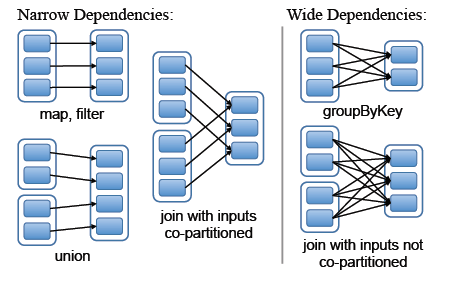
\includegraphics[width=\textwidth]{images/RDDdependencies.png}
% \end{frame}

% \begin{frame}[fragile]
% \frametitle{Working with Key-value pairs}
% \begin{lstlisting}{title=Key-value pairs in different languages}
% pair = (a, b)
%     pair[0] # => a 
%     pair[1] # => b
% val pair = (a, b)
%     pair._1 // => a
%     pair._2 // => b
% Tuple2 pair = new Tuple2(a, b); 
%     pair._1 // => a
%     pair._2 // => b
% \end{lstlisting}
% \end{frame}


\section{Using Spark}

\begin{frame}[fragile]
  \frametitle{Local deployment using docker-compose}
  
  \center
{  \Large
\only<1>{
  Get the repo
}
  
\only<2>{
  Move to the repo
}
\only<3>{
  Run all the containers
}
\only<4>{
  Launch spark-shell inside the master container
}
}
\vfill

  \begin{lstlisting}[basicstyle=\ttfamily,linebackgroundcolor={
      \btLstHL<1>{1}%
      \btLstHL<2>{2}%
      \btLstHL<3>{3}%
      \btLstHL<4>{4}%
    }]
git clone http://github.com/gettyimages/docker-spark
cd docker-spark
docker-compose up
docker exec -it dockerspark_master_1 bin/spark-shell 
\end{lstlisting}

\end{frame}


\begin{frame}[fragile]
  \frametitle{Demo}
  \centering
\href{https://asciinema.org/a/92977}{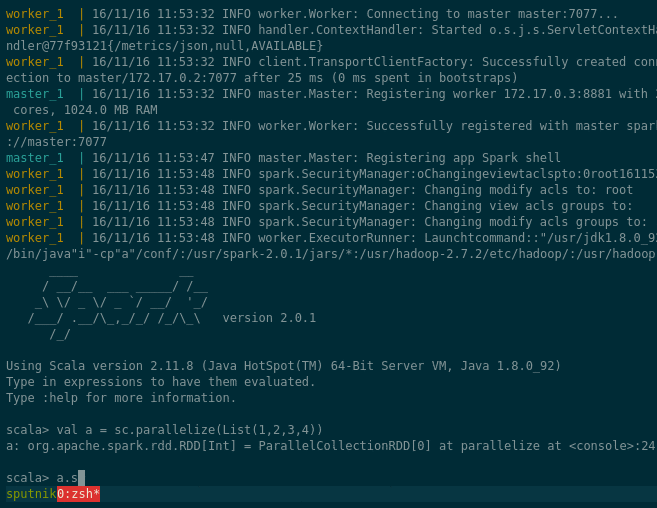
\includegraphics[width=\textwidth]{gif/sparkrepl-thumb.png}}

\end{frame}
\begin{frame}[fragile]{Compose.yml Master}
\vspace{-2em} % Avoid overlapping with footer
\begin{lstlisting}[basicstyle=\ttfamily,language={},linebackgroundcolor={
    \btLstHL<1>{2}%
    \btLstHL<2>{3}%
    \btLstHL<3>{11}%
    \btLstHL<4>{12}%
    }]
master:
  image: gettyimages/spark
  command: bin/spark-class org.apache.spark.deploy.master.Master -h master
  hostname: master
  environment:
    MASTER: spark://master:7077
    SPARK_CONF_DIR: /conf
    SPARK_PUBLIC_DNS: localhost
    ... bunch of ports ...
  volumes:
    - ./conf/master:/conf
    - ./data:/tmp/data
  \end{lstlisting}
\end{frame}
\begin{frame}[fragile]{Compose.yml Worker}
\vspace{-2em} % Avoid overlapping with footer
\begin{lstlisting}[language={},basicstyle=\ttfamily,linebackgroundcolor={
    \btLstHL<1>{2}%
    \btLstHL<2>{3}%
    \btLstHL<3>{12,13}%
    \btLstHL<4>{6-8}%
    }]
worker:
  image: gettyimages/spark
  command: bin/spark-class org.apache.spark.deploy.worker.Worker spark://master:7077
  hostname: worker
  environment:
    SPARK_CONF_DIR: /conf
    SPARK_WORKER_CORES: 2
    SPARK_WORKER_MEMORY: 1g
  links:
    - master
  volumes:
    - ./conf/worker:/conf
    - ./data:/tmp/data
    \end{lstlisting}
\end{frame}
\begin{frame}[fragile]
  \frametitle{Useful info}
  \begin{itemize}
  \item ./data folder is mounted as /tmp/data
    \begin{itemize}
    \item Copy your datasets there
    \item Load them in the shell: \texttt{sc.textFile("/tmp/data/...")}
    \end{itemize}
  \item Master Web UI (localhost:8080)
  \item Worker Web UI (localhost:8081)
  \item REPL Web UI (localhost:4040 when launched)
    \end{itemize}
\textbf{A word of caution}: as any other app, the shell reserves resources on startup, whether you are using them or not.
\end{frame}

\begin{frame}[fragile]
  \frametitle{Applications}
  Steps:
  \begin{itemize}
    \item Write the code
    \item Compile the jar
    \item Make your data available to every node in the cluster
    \item Submit it to your cluster 
  \end{itemize}
\end{frame}
\begin{frame}[fragile]
  \frametitle{Writing applications}
    \begin{lstlisting}[title=Example application,basicstyle=\ttfamily]
import org.apache.spark.SparkContext
import org.apache.spark.SparkContext._
import org.apache.spark.SparkConf

object SparkWordCount {
  def main(args: Array[String]) {
    // create Spark context with Spark configuration
    val sc = new SparkContext(new SparkConf().setAppName("Spark Example"))
  ... Your program ...
}
\end{lstlisting}
\end{frame}

\begin{frame}[fragile]
  \frametitle{Running an aplication}
    \begin{lstlisting}[language={},numbers=none]
./bin/spark-submit --class <main-class> \
                     --master <master-url> \
                     --deploy-mode <deploy-mode> \
                     --conf <key>=<value> \
                     ... # other options
                     <application-jar> \
                     [application-arguments]
\end{lstlisting}
\end{frame}

\section{Full examples}

\begin{frame}[fragile]
  \frametitle{Word frequency in wikipedia, revisited}
  \begin{lstlisting}[title=Spark,basicstyle=\ttfamily,linebackgroundcolor={\color{orange!30}}]
val wiki = sc.textFile("Wikipedia.txt")
val counts = wiki.flatMap(line=> line.split(" ")
                map(word => (word, 1)))
                reduceByKey(_ + _)
\end{lstlisting}

\begin{lstlisting}[title=Pure scala,basicstyle=\ttfamily]
val wiki = scala.io.Source.fromFile("Wiki").getLines
wiki.flatMap(line=> line.split(" "))
      map(x=>(x, 1)).toList
      groupBy(x => x._1)
      map({case (k, v) =>
            (k, v.foldLeft(0)((a, b) => a+b._2)))
  \end{lstlisting}
\end{frame}

\begin{frame}[plain]
  \center
  \huge{Shall we try it in the shell?}
\end{frame}

{
  \pagecolor{black}
  \usebackgroundtemplate{\vbox to \paperheight{\vfil\hbox to \paperwidth{\hfil
\includegraphics[height=\paperheight]{images/justwaithere.jpg}\hfil}\vfil}}%

\begin{frame}[plain]
\end{frame}
}

\begin{frame}
  \frametitle{Spark is not magic}
  \begin{itemize}
    \item We still have to add more resources
    \item Caching may cause the spark version to use \textbf{more memory} (this can be configured)
  \end{itemize}
  \center
  \pause
  \huge{However, it allows us to scale our application}

\end{frame}


% \begin{frame}
%   \frametitle{Word count}
% 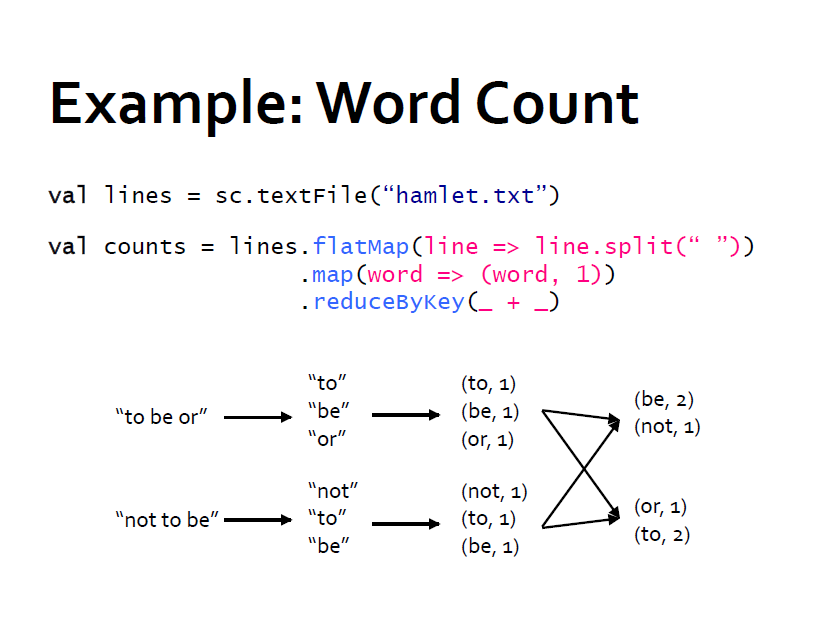
\includegraphics[width=\textwidth]{images/wordcount.png}
% \end{frame}

\begin{frame}[fragile]
  \frametitle{Page rank}

  \begin{columns}
    \column{0.5\textwidth}
    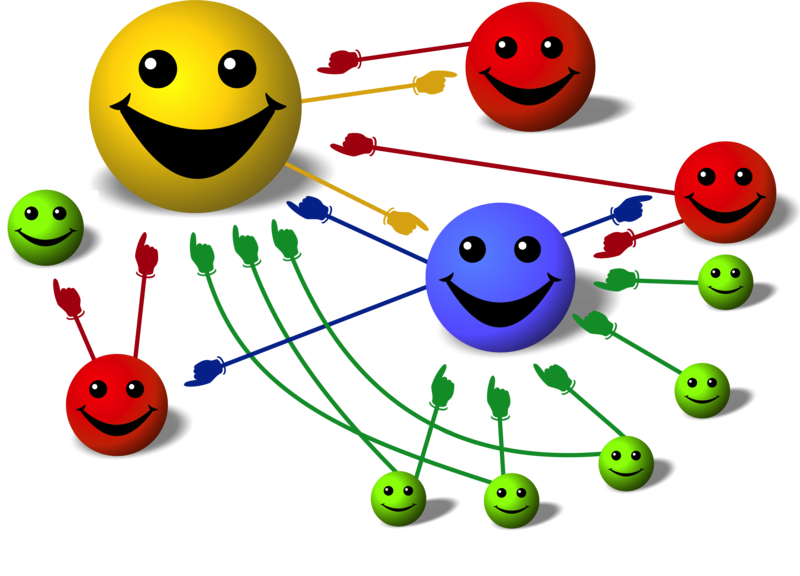
\includegraphics[width=\textwidth]{images/pagerank.png}
    \column{0.5\textwidth}
    \begin{itemize}
    \item Created by Google
    \item Rank given by links and their importance
    \item Iterative (Perfect for Spark!)
    \end{itemize}
  \end{columns}
  \begin{centering}

$
 \text{PageRank of site} = \sum \frac{\text{Page rank of inbound link}}{\text{Number of links on that page}}
$

OR

$
 PR(u) = (1-d)+d\times \sum \frac{PR(v)}{N(V)}
$

\end{centering}
\end{frame}

{
  \pagecolor{white}
  \usebackgroundtemplate{\vbox to \paperheight{\vfil\hbox to \paperwidth{\hfil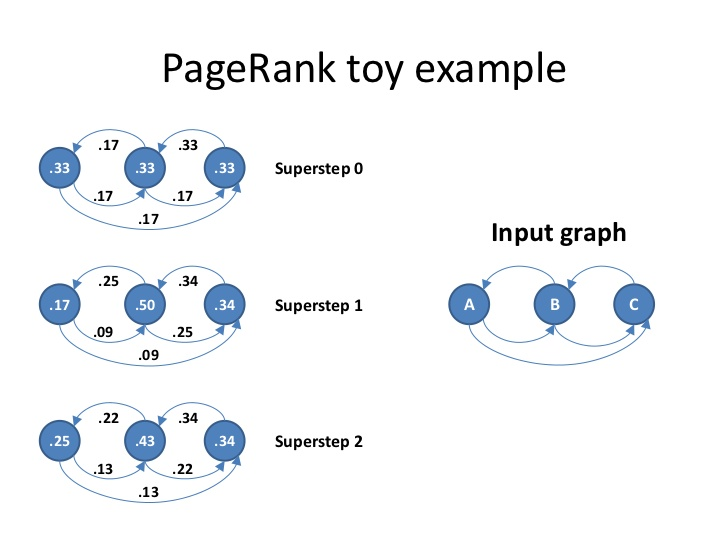
\includegraphics[height=\paperheight]{images/pageranktoy.jpg}\hfil}\vfil}}%

\begin{frame}[plain]
% 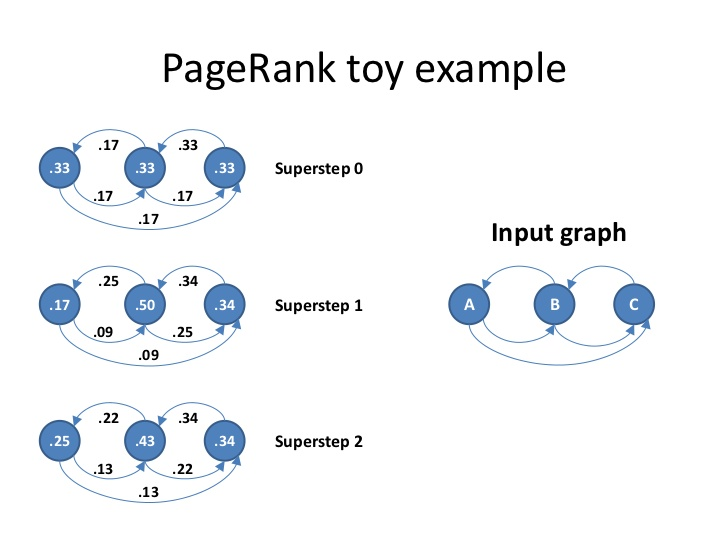
\includegraphics[width=\textwidth]{images/pageranktoy.jpg}
\footnote{\url{http://www.slideshare.net/sscdotopen/large-scale}}

\end{frame}
}

\begin{frame}
\frametitle{Page rank (code)}
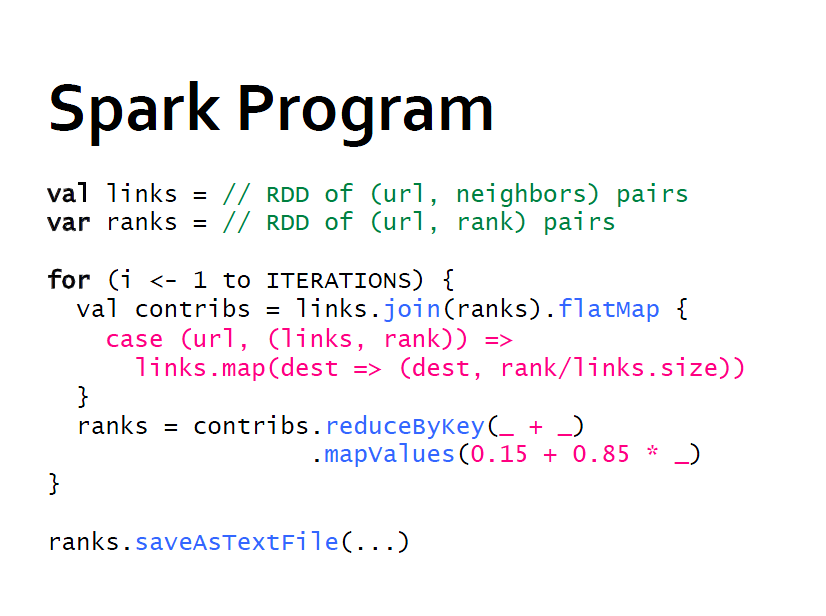
\includegraphics[width=\textwidth]{images/example.png}
\end{frame}

\section*{Next week}

\begin{frame}{Next week}
  \begin{itemize}
  \item Advanced Spark configuration
  \item Multiple hosts
  \item Spark ecosystem
  \item More examples in IBM BlueMix
  \end{itemize}
\end{frame}

\section{Acknowledgements and useful links}

\begin{frame}
  \begin{itemize}
\item \href{http://spark.apache.org/docs/latest/programming-guide.html}{Spark programming guide}
\item \href{https://databricks.com/blog/2016/01/04/introducing-apache-spark-datasets.html}{Databricks introducing apache spark datasets}
\item \href{https://www.safaribooksonline.com/library/view/data-analytics-with/9781491913734/ch04.html}{Data Analytics with Hadoop: In-Memory Computing with Spark}
  \end{itemize}
\end{frame}

\end{document}
